\documentclass[10pt]{article}

\input{/Users/gabesekeres/Dropbox/LaTeX_Docs/pset_preamble.tex}

\course{ECON 6140}
\pset{7}
\begin{document}
\maketitle

\textbf{Authors:} Gabe Sekeres and Finn Ye

\textbf{NetIDs:} \href{https://www.google.com/search?q=i+object+to+this+requirement+and+am+participating+under+protest&oq=i+object+to+this+requirement+and+am+participating+under+protest&gs_lcrp=EgZjaHJvbWUyBggAEEUYOTIHCAEQIRiPAjIHCAIQIRiPAtIBCTIwNjk2ajBqN6gCALACAA&sourceid=chrome&ie=UTF-8}{gs754} and fy55

\textbf{\textit{n.b.}} All code is below, in the \href{sec:code}{code section}.

\begin{enumerate}
	\item First, note that there is a production subsidy in place of $\tau = \frac{1}{\varepsilon}$ such that \[- \frac{U_{n,t}}{U_{c,t}} = \frac{W_t}{P_t} = \frac{W_t}{\mathcal{M}\frac{W_t(1-\tau)}{MPN_t}} = MPN_t\]Following the notes and substituting in the respective rules into the dynamic IS equation, we get that \[\tilde{y}_t = \expect_t\{\tilde{y}_{t+1}\} - \frac{1}{\sigma} (\rho + \phi_\pi\pi_t + \phi_y\tilde{y}_t - \expect_t\{\pi_{t+1}\} - \rho + \sigma(1-\rho_a)\psi_{ya} a_t - (1-\rho_z)z_t)\]We will conjecture that our two variables of interest take the form \begin{align*} \pi_t &= \psi_{\pi a} a_t + \psi_{\pi z} z_t \\ \tilde{y}_t &= \psi_{y a} a_t + \psi_{y z} z_t\end{align*}So under rational expectations, since both $a_t$ and $z_t$ are AR(1) processes and $\expect[\varepsilon_t^a] = \expect[\varepsilon_t^z] = 0$, we have that \begin{align*} \expect\{\pi_{t+1}\} &= \psi_{\pi a}\rho_a a_t + \psi_{\pi z}\rho_z z_t \\\expect\{\tilde{y}_{t+1}\} &= \psi_{y a}\rho_a a_t + \psi_{y z}\rho_z z_t\end{align*}Substituting the conjectured solution into our two equations of interest, we get \begin{align*} \psi_{\pi a} a_t + \psi_{\pi z} z_t &= \beta \parl \psi_{\pi a}\rho_a a_t + \psi_{\pi z}\rho_z z_t \parr + \kappa \parl  \psi_{y a} a_t + \psi_{y z} z_t\parr \\ \psi_{y a} a_t + \psi_{y z} z_t &= \psi_{y a}\rho_a a_t + \psi_{y z}\rho_z z_t -  \frac{1}{\sigma} (\phi_\pi(\psi_{\pi a} a_t + \psi_{\pi z} z_t) + \phi_y(\psi_{y a} a_t + \psi_{y z} z_t) \\ &\;\qquad - (\psi_{\pi a}\rho_a a_t + \psi_{\pi z}\rho_z z_t) + \sigma(1-\rho_a)\psi_{ya} a_t - (1-\rho_z)z_t)\end{align*}Isolating the shocks, we have that\begin{align*} a_t \parl  \psi_{\pi a} - \psi_{\pi a}\rho_a - \kappa \psi_{ya}\parr + z_t\parl  \psi_{\pi z} - \psi_{\pi z}\rho_z - \kappa \psi_{yz}\parr &= 0 \\ a_t \parl \psi_{ya} - \psi_{ya}\rho_a + \frac{\psi_{\pi a} \phi_\pi + \psi_{ya}\phi_y - \psi_{\pi a} \rho_a}{\sigma} +(1-\rho_a)\psi_{ya}\parr + &\;\\ z_t \parl  \psi_{yz} - \psi_{yz}\rho_z + \frac{\psi_{\pi z} \phi_\pi + \psi_{yz}\phi_y - \psi_{\pi z} \rho_z - (1-\rho_z)}{\sigma}\parr &= 0\end{align*}Since we need these equations to hold for each possible shock in steady state, we will fix everything inside the parentheses to be zero. This will give is four linear equations in our four unknowns. We have: \begin{align*}   (1-\rho_a)\psi_{\pi a} - \kappa \psi_{ya} &= 0 \\ (1-\rho_z) \psi_{\pi z} - \kappa \psi_{yz} &= 0 \\   \frac{\phi_\pi-\rho_a}{\sigma}\psi_{\pi a} + \parl 2(1-\rho_a) + \frac{\phi_y}{\sigma}\parr \psi_{ya} &= 0 \\   \frac{\phi_\pi-\rho_z}{\sigma}\psi_{\pi z} + \parl 1-\rho_z + \frac{\phi_y}{\sigma}\parr \psi_{yz} &= \frac{1-\rho_z}{\sigma}\end{align*}Putting everything in matrix form, this becomes \[\underbrace{\matrixc{1-\rho_a & -\kappa & 0 & 0 \\ 0 & 0 & 1-\rho_z & -\kappa \\ \frac{\phi_\pi - \rho_a}{\sigma} & 2 - 2\rho_a + \frac{\phi_y}{\sigma} & 0 & 0 \\ 0 & 0 & \frac{\phi_\pi - \rho_z}{\sigma} & 1-\rho_z + \frac{\phi_y}{\sigma}}}_{A} \cdot \matrixc{\psi_{\pi a} \\ \psi_{ya} \\ \psi_{\pi z} \\ \psi_{yz}} = \matrixc{0 \\ 0 \\ 0 \\ \frac{1-\rho_z}{\sigma}}\]So we have that\[\matrixc{\psi_{\pi a} \\ \psi_{ya} \\ \psi_{\pi z} \\ \psi_{yz}} = A^{-1} \cdot \matrixc{0 \\ 0 \\ 0 \\ \frac{1-\rho_z}{\sigma}}\]Putting everything together in Julia, and adding the actual values of the coefficients, recalling from the notes that $\kappa = \parl \sigma + \frac{\varphi + \alpha}{1-\alpha}\parr \frac{(1-\theta)(1-\beta\theta)}{\theta} \frac{1-\alpha}{1-\alpha+\alpha\varepsilon}$, we get that: \[\matrixc{\psi_{\pi a} \\ \psi_{ya} \\ \psi_{\pi z} \\ \psi_{yz}} = \matrixc{0 \\ 0 \\ 0.09823 \\ 0.26785}\]The first two being zero is strange compared to what we had in class, but relates to the fact that the natural rate of interest is itself a function of $\psi_{ya}$. This means that the only way we can hold in steady state is if neither inflation nor output respond to the log productivity shocks. 
	\item I simulated the model over 100 periods, and got the following time series data: \begin{figure}[H] \centering 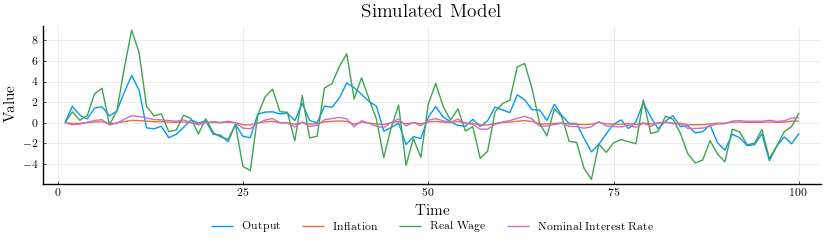
\includegraphics[width=15cm]{macro_hw7_code/2_simulated_model.png}\end{figure}
	\item I simulated a single firm over 100 periods, only letting them change their price $(1-\theta)$ of the time (using a uniform random variable over the unit interval), and the firm's price was in the following figure: \begin{figure}[H] \centering 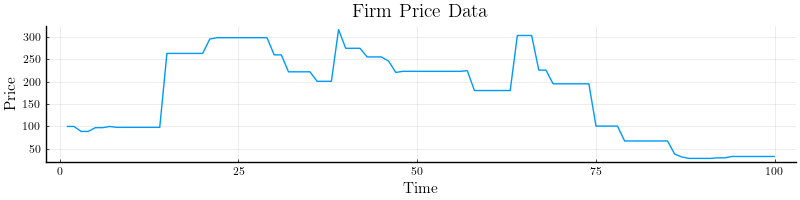
\includegraphics[width=15cm]{macro_hw7_code/3a_firm_price_data.png} \end{figure} The firm changed its price 28 times, and the average price duration was 2.3537 periods. This is similar to what we would expect from $\theta$, of changing the price 25 times with an average duration of 3 periods. Plotting the price of firm $j$ with respect to the aggregate price gives us \begin{figure}[H]\centering 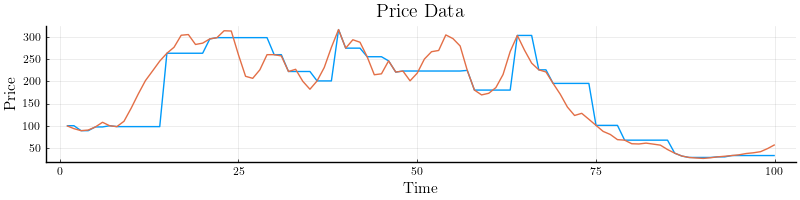
\includegraphics[width=15cm]{macro_hw7_code/3b_price_data.png} \end{figure}Plotting the output of the firm with respect to the aggregate output gives us \begin{figure}[H] \centering 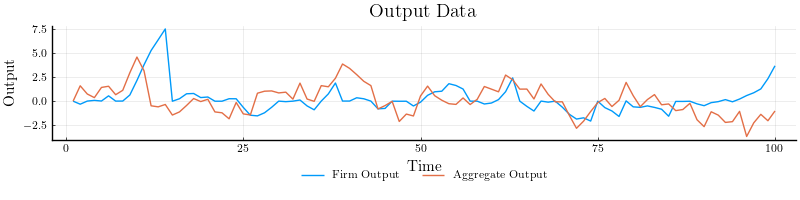
\includegraphics[width=15cm]{macro_hw7_code/3c_output_data.png}\end{figure}Plotting the marginal cost gives us \begin{figure}[H] \centering 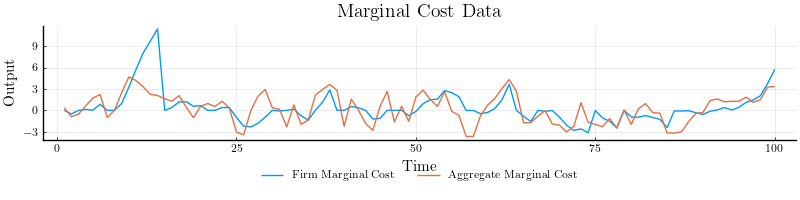
\includegraphics[width=15cm]{macro_hw7_code/3d_marginal_cost_data.png} \end{figure} We conclude that the output and marginal cost are very correlated, anda are inversely correlated with the price levels.
	\item I redid the earlier analysis for the three changed parameterizations: \begin{enumerate} \item We set $\varepsilon = 10$. The plots we generated are: \begin{figure}[H] \centering 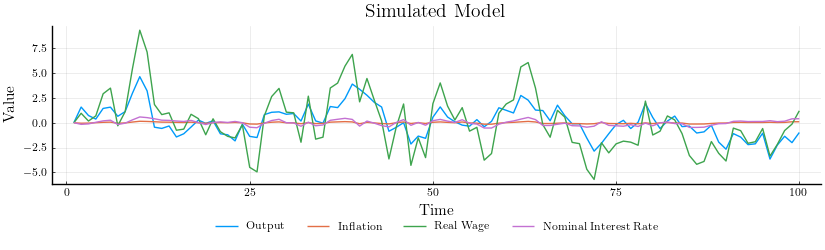
\includegraphics[width=15cm]{macro_hw7_code/4a2_simulated_model.png}\end{figure}\begin{figure}[H] \centering 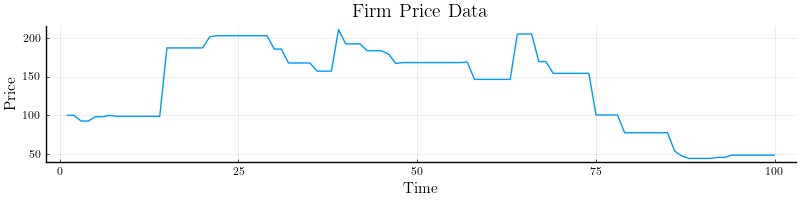
\includegraphics[width=15cm]{macro_hw7_code/4a3a_firm_price_data.png}\end{figure}\begin{figure}[H] \centering 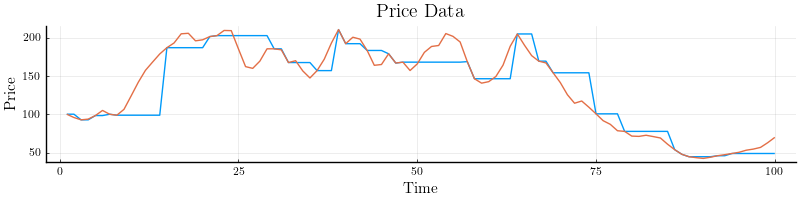
\includegraphics[width=15cm]{macro_hw7_code/4a3b_price_data.png}\end{figure}\begin{figure}[H] \centering 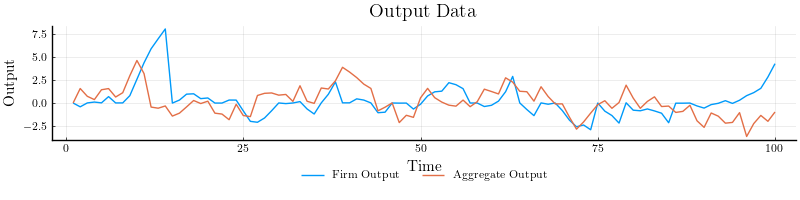
\includegraphics[width=15cm]{macro_hw7_code/4a3c_output_data.png}\end{figure}\begin{figure}[H] \centering 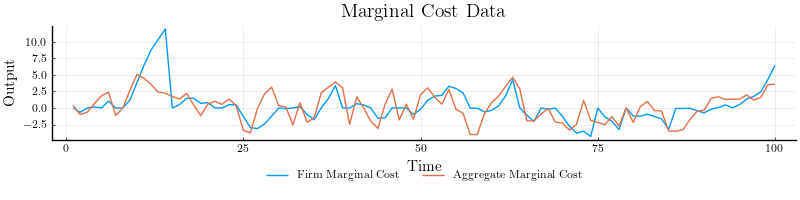
\includegraphics[width=15cm]{macro_hw7_code/4a3d_marginal_cost_data.png}\end{figure} We found that the variance of inflation was lower, the variance of output was slightly higher but basically the same, and that the variance of marginal cost increased substantially. We conclude that increasing $\varepsilon$ decreases the change in inflation decreases but that the marginal cost gets rougher period-to-period. \item We set $\alpha = 0$. The plots we generated are: \begin{figure}[H] \centering 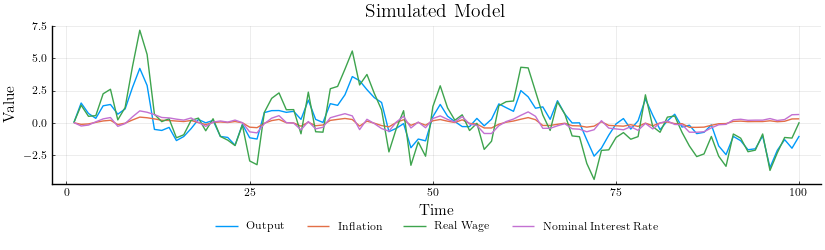
\includegraphics[width=15cm]{macro_hw7_code/4b2_simulated_model.png}\end{figure}\begin{figure}[H] \centering 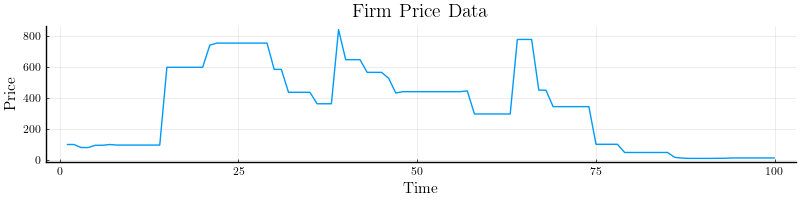
\includegraphics[width=15cm]{macro_hw7_code/4b3a_firm_price_data.png}\end{figure}\begin{figure}[H] \centering 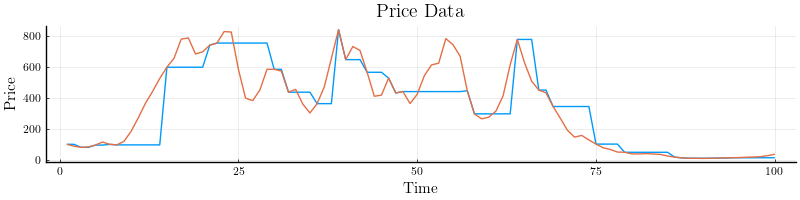
\includegraphics[width=15cm]{macro_hw7_code/4b3b_price_data.png}\end{figure}\begin{figure}[H] \centering 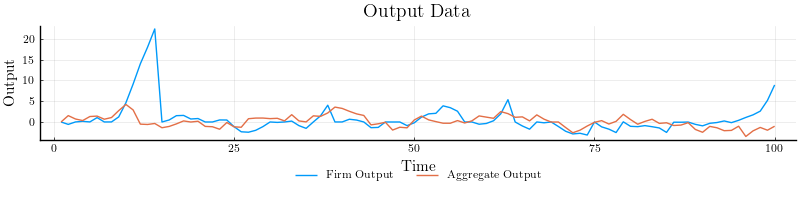
\includegraphics[width=15cm]{macro_hw7_code/4b3c_output_data.png}\end{figure}\begin{figure}[H] \centering 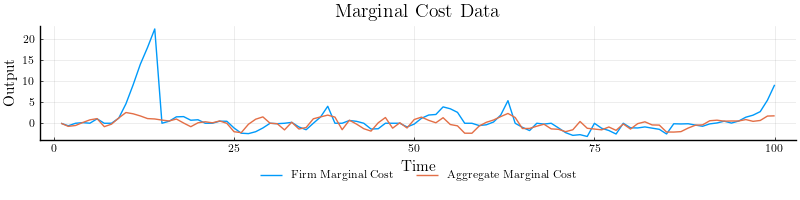
\includegraphics[width=15cm]{macro_hw7_code/4b3d_marginal_cost_data.png}\end{figure} We found that the variance of everything except for output increases, and marginal cost increased massively in variance. We can see from the plots that there is a big spike in each and then a decrease back to relatively stable levels. \item We set $\phi_\pi = 10$ and $\phi_y = 0$. The plots we generated are: \begin{figure}[H] \centering 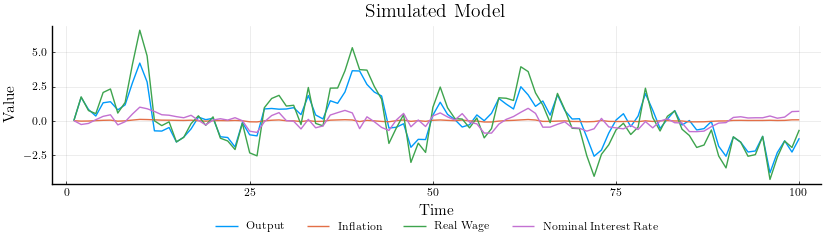
\includegraphics[width=15cm]{macro_hw7_code/4c2_simulated_model.png}\end{figure}\begin{figure}[H] \centering 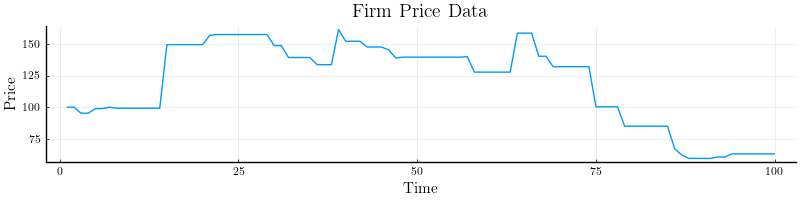
\includegraphics[width=15cm]{macro_hw7_code/4c3a_firm_price_data.png}\end{figure}\begin{figure}[H] \centering 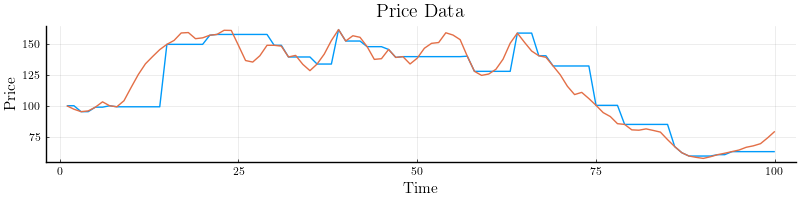
\includegraphics[width=15cm]{macro_hw7_code/4c3b_price_data.png}\end{figure}\begin{figure}[H] \centering 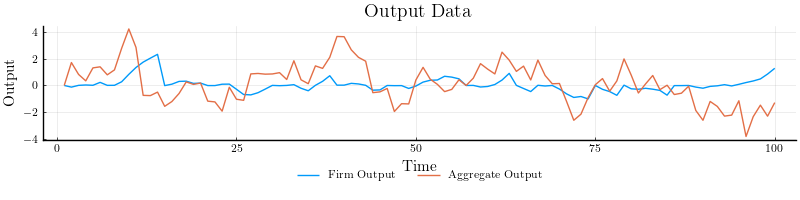
\includegraphics[width=15cm]{macro_hw7_code/4c3c_output_data.png}\end{figure}\begin{figure}[H] \centering 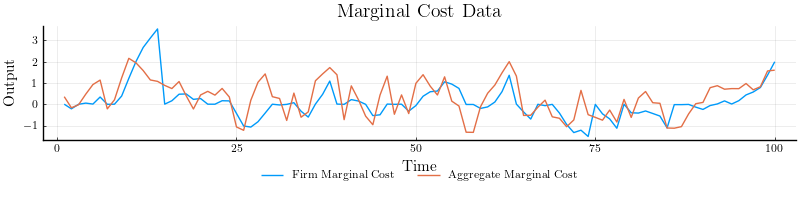
\includegraphics[width=15cm]{macro_hw7_code/4c3d_marginal_cost_data.png}\end{figure} We found that the variance of inflation and marginal cost both massively decreased, but that output variance did not change that much at all. This can be seen in the plots, where it's quite spiky. \end{enumerate}
	\item We calculated the price path using the expression \[p\opt_t = \frac{1-\alpha}{1-\alpha + \alpha\varepsilon} \parl \sigma + \frac{\varphi + \alpha}{1-\alpha} \tilde{y}_t\parr + \pi_t\]We got that the perfectly flexible firm would charge the same as exactly the aggregate price levels. This seems wrong, since the question seems to be guiding us towards a ``no'' answer, but we don't know what's going on here. The prices are:\begin{figure}[H] \centering 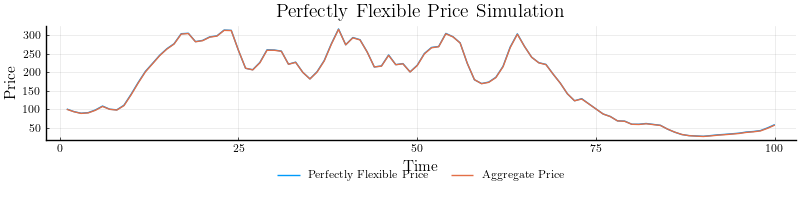
\includegraphics[width=15cm]{macro_hw7_code/5_perfectly_flexible_price_simulation.png}\end{figure}
\end{enumerate}


\newpage
\section*{Code Section}\label{sec:code}

The code was:
\lstinputlisting[language=Julia]{macro_hw7_code/functions.jl}
\lstinputlisting[language=Julia]{macro_hw7_code/main.jl}


\end{document}